\documentclass[11pt,titlepage,a4paper]{report}

%INCLUSIONE PACCHETTI
%---------------------------------------------
\usepackage[italian]{babel}
\usepackage{fancyhdr}
\usepackage{graphicx}
\graphicspath{{./pics/}} % cartella di salvataggio immagini

% STILE DI PAGINA
%---------------------------------------------
\pagestyle{fancy}
\renewcommand{\sectionmark}[1]{\markright{\thesection.\ #1}}
\lhead{\nouppercase{\rightmark}}
\rhead{\nouppercase{\leftmark}}
\renewcommand{\chaptermark}[1]{%
\markboth{\thechapter.\ #1}{}}

%Ridefinisco lo stile plain della pagina
\fancypagestyle{plain}{%
	\lhead{
\includegraphics[height=50pt]{logo.eps}}
	\chead{}
	\rhead{HappyCode inc \\ happycodeinc@gmail.com}
	\lfoot{BR-jsys}
	\rfoot{\dt - \lv}
	\cfoot{\thepage}
	\renewcommand{\headrulewidth}{1pt}
	\renewcommand{\footrulewidth}{1pt}
}

\begin{document}

%definizione variabili 
\newcommand{\lv}{ 0.3 } % latest version
\newcommand{\dt}{ Definizione del Prodotto }% Document title
\newcommand{\Glossario}{ Glossario.1.4.pdf }
%fine definizione variabili
\newcommand{\br}{business rule }
\newcommand{\brs}{business rules }
\newcommand{\bo}{business object }
\newcommand{\bos}{business objects }
\newcommand{\re}{repository}
\newcommand{\brp}{BusinessRuleParser }
\newcommand{\brl}{BusinessRuleLexer }
\newcommand{\BR}{BusinessRule }


\hyphenation{glos-sa-rio es-pli-ci-to ve-ri-fi-ca-re re-po-si-to-ry se-gna-la-ta coe-ren-za}
\begin{titlepage}\begin{center}
\vspace*{0.5in}

\includegraphics{logo.eps}
\vspace*{0.2in} \\
{\Large \textbf{BR-jsys}}
{\Large \emph{business rules} per sistemi gestionali in architettura J2EE } 
\vspace{2in} \\
\Huge \textsc{ \dt }
\par\rule{10cm}{0.4pt} \par {\large Versione \lv - \today} \\
\end{center}\end{titlepage}
\vspace*{0.5in}

\begin{center}
\thispagestyle{plain}
\begin{table}[htbp]
\large{
\begin{tabular}{l}
\Large{\textbf{\textsf{Capitolato: ''BR-jsys``}}} \\
\begin{tabular}{||p{6cm}||p{6cm}||}
\hline
\textbf{Data creazione:} & 18/11/2007 \\ \hline
\textbf{Versione:} & \lv \\ \hline
\textbf{Stato del documento:} & Formale, esterno \\ \hline
% ----------------------------------------------------------------------------autori
\textbf{Redazione:} & Carraro Filippo, Luca Appon \\ \hline
\textbf{Revisione:} & Michele Bortolato   \\ \hline
\textbf{Approvazione:}  & Luca Appon \\ \hline
\end{tabular} \\
\end{tabular}
}
\end{table}

\begin{table}[hbtp]
\large{
\begin{tabular}{l}
\Large{\textbf{\textsf{Lista di distribuzione}}} \\
\begin{tabular}{||p{6cm}||p{6cm}||} \hline
%  -------------------------------------------------------------lista di distribuzione
{Elena Trivellato}& Responsabile di progetto \\ \hline 
{Filippo Carraro}& Progettista \\ \hline
{Alessia Trivellato, Michele Bortolato}& Analisti \\ \hline
{Marco Tessarotto}& Verificatore \\ \hline
{Tullio Vardanega, Renato Conte}& Committente \\ \hline 
{Zucchetti S.r.l}& Azienda proponente\\ \hline
\end{tabular} \\
\end{tabular}
}
\end{table}
\begin{table}[hbtp]
\large{
\begin{tabular}{l}
\Large{\textbf{\textsf{Diario delle modifiche}}} \\
\begin{tabular}{||p{2cm}||p{3.5cm}||p{6cm}||} \hline
%-------------------------------------------------------------------------------diario modifiche
\textbf{Versione} & \textbf{Data rilascio} & \textbf{Descrizione} \\ \hline
0.3 & 2008/02/05 & Aggiunta del nome del file nel modello di documento.\\ \hline
0.2 & 26/01/2007 & Documento sottoposto a revisionamento automatico.\\ \hline
0.1 & 25/01/2007 & Stesura preliminare del documento. \\ \hline

\end{tabular} \\
\end{tabular}

}
\end{table}
\end{center}
\newpage



\chapter{Introduzione}
\section{Scopo del documento}
Il seguente documento ha lo scopo di descrivere l'architettura logica prodotta al termine della fase di progettazione architetturale, esso descrive in dettaglio i campi dati e i metodi appartenenti alle singole componenti del sistema.
\section{Scopo del prodotto}
Per lo scopo del prodotto si faccia riferimento al documento di Analisi dei Requisiti.
\section{Glossario}
Viene fornito come documento esterno chiamato Glossario.1.4.pdf.

\section{Riferimenti}
\begin{itemize}
\item Capitolato d'appalto concorso per sistema ``BR-jsys''
\item Verbale dell'incontro con il committente ``Incontro2007-11-22.pdf''
\item Verbale dell'incontro con il committente ``Incontro2008-02-05.pdf''
\item ``Analisi dei Requisiti''
\item ``Piano di Qualifica''
\item ``Norme di Progetto''
\item ``Specifica tecnica''
\item ``Ingegneria del Software'' 8a edizione - Ian Sommerville
\item ``The Definitive ANTLR Reference''
\end{itemize}
\chapter{Standard di progetto}
\section{Standard di progettazione architetturale}
Per le rappresentazioni grafiche dell'architettura del nostro sistema, ci baseremo sulle regole definite da UML 2.1.
\section{Standard di documentazione del codice}
Le specifiche per la documentazione del codice sono descritte nel documento %serve il nome giusto delle norme di progetto.
\section{Standard di denominazione di entit\`a e relazioni}

\section{Standard di programmazione}
\section{Strumenti di lavoro}
%annotare per le sezioni sopra le norme di codicfica
\chapter{Specifica delle componenti}
\section{GUI}
\subsection{Diagramma delle classi}
\begin{center}
%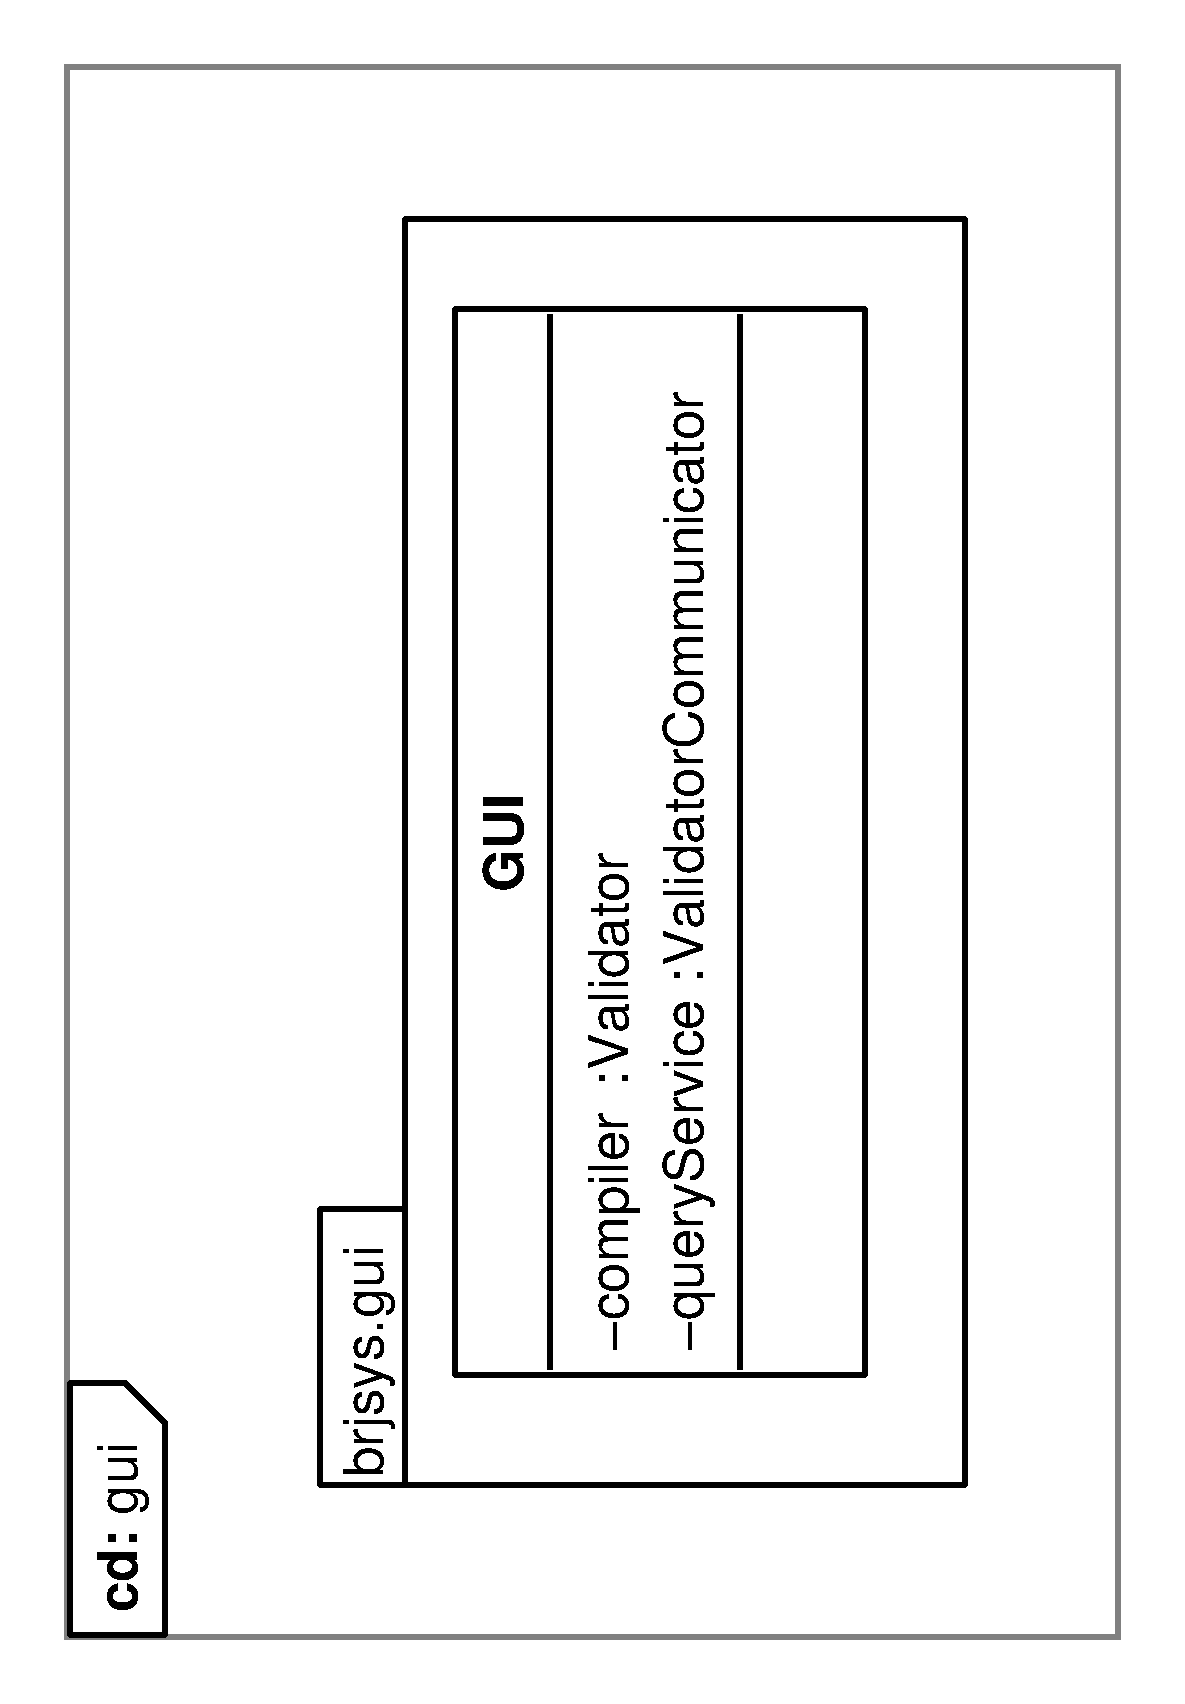
\includegraphics[width=0.5\textwidth, angle=-90]{DiagrammaClassi/gui.eps}
\end{center}
\subsection{Gui}
\subsubsection{Tipo, obiettivo e funzione del componente}
Questa componente fornisce all'utente un interfaccia minimale consentendogli di effettuare le operazioni di cancellazione, e di querying sul \re.
Nel caso di esecuizone di una query definita dall'utente verranno fornite inoltre informazioni relative ai tempi d'esecuzione.
Questa componente viene realizzata tramite una singola classe java.
\subsubsection{Relazioni d'uso di altre componenti}
Questa componente utilizza:
\begin{itemize}
 \item \BR per dichiarare una nuova \br da spedire al validatore;
 \item Validator per effettuare la validazione di una \br;
 \item GUICommunicator che verr\`a trattato successivamente.
\end{itemize}
\subsubsection{Interfacce con e relazioni di uso da altre componenti}
Nessuna.
\subsubsection{Attivit\`a svolte e dati trattati}
La componente possiede i campi dato necessari per comunicare con le copmponente validatore e con la componente DBMS.
\begin{center}
% use packages: array
\begin{tabular}{||p{6cm}||p{6cm}||} \hline
\hline
Attributo & Descrizione \\  \hline
-compiler:Validator & Rappresenta il validatore per le \br \\ \hline
-repository:GUICommunicator & Collega la componente al DBMS consentendogli di effettuare le Query.\\ \hline
\end{tabular}
\end{center}
\begin{center}
\begin{tabular}{||p{6cm}||p{6cm}||} \hline
\hline
Metodo & Descrizione \\  \hline
\underline{+main(args:String[]):Validator} & Metodo standard in java per l'avvio dell'applicazione incaricher\`a di creare un oggetto Gui\\ \hline
+Gui() & Costruttore per Gui.\\ \hline
\end{tabular}
\end{center}


\section{Validatore}
\subsection{Diagramma delle classi}
\begin{center}
%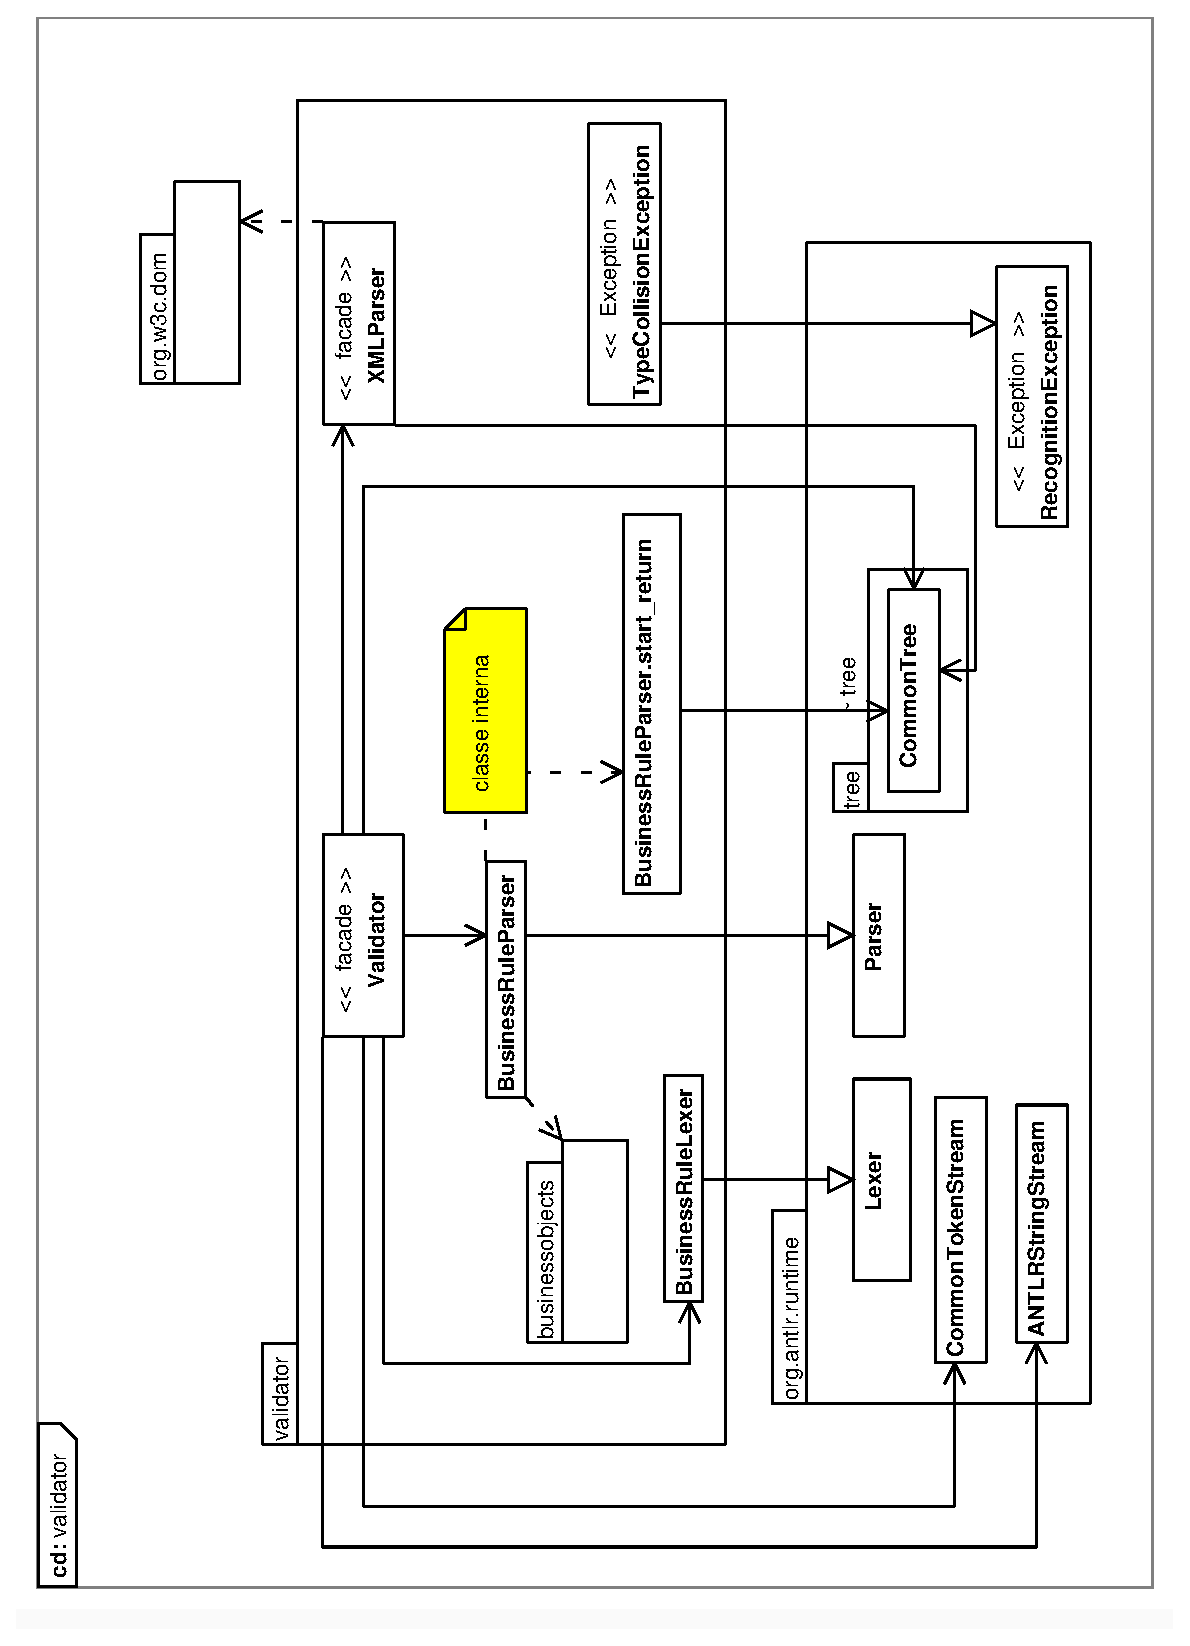
\includegraphics[width=0.6\textwidth, angle=-90]{DiagrammaClassi/validator.eps}
\end{center}
\subsection{Validator}%facade!!!->va descritto
\subsubsection{Tipo, obiettivo e funzione del componente}
Questa componente effettua la validazione di una \br senza far fare all'utilizzatore tutte le singole operazioni di compilazione.
Validator ha il ruolo di \textit{fa\c{c}ade} in quanto fornisce un interfaccia unificata che riesce a gestire in maniera semplice ed immediata le operazioni di compilazione e di insermento che avremmo altrimenti dovuto riportare direttamente dove la cmponente GUI lo richiedesse.
\subsubsection{Relazioni d'uso di altre componenti}
Validator usa le componenti \brp, \brl, XMLParser e ValidatorCommunicator che verranno descritte in seguito.
\subsubsection{Interfacce con e relazioni di uso da altre componenti}
Validator \`e in relazione con la componente GUI per permettere la validazione.
\subsubsection{Attivit\`a svolte e dati trattati}
La componente deve occuparsi della validazione e del successivo inserimento nel \re.
\begin{center}
\begin{tabular}{||p{6cm}||p{6cm}||} \hline
\hline
Attributo & Descrizione \\  \hline
-repository:ValidatorCommunicator & Collega la componente al DBMS per inserire la \br validata nel \re.\\ \hline
\end{tabular}
\end{center}
\begin{center}
\begin{tabular}{||p{6cm}||p{6cm}||} \hline
\hline
Metodo & Descrizione \\  \hline
+Validator() & Costruttore di Validator\\ \hline
+validate(rule: BusinessRule ):boolean \lbrace throws\phantom{c} RecognitionException \rbrace& Unico metodo della componente che ricevuto in ingresso una \br ne effettua la validazione. qualora si verificassero errori in fase di compilazione si restituir\`a un eccezzione che verr\`a gestita dal chiamante. Se la \br viene inserita il metodo ritorner\`a \textit{true}, ritornero \textit{false} se la regola ha un nome che \`e gi\`a presente nel \re.\\ \hline
\end{tabular}
\end{center}

\subsection{BusinessRuleLexer}
\subsubsection{Tipo, obiettivo e funzione del componente}
Questa componente, derivata da org.antlr.runtime.Lexer, non \`e altro che una classe wrapper per la stringa che rappresenta la \br che aggiunge ad essa funzionalit\`a necessarie per il successivo parsing.
\subsubsection{Relazioni d'uso di altre componenti}
Nessuna.
\subsubsection{Interfacce con e relazioni di uso da altre componenti}
La componente BusinessRuleParser necessita la componente BusinessRuleLexer che verr\`a approfondita successivamente.
\subsubsection{Attivit\`a svolte e dati trattati}
La componente, che viene generata tramite un generatore di parser, dispone di numerosi campi dato per identificare i token della grammatica nonch\`e vari metodi per la loro gestione, in effettivo si dovra' usare soltanto il suo costruttore.
\begin{center}
\begin{tabular}{||p{6cm}||p{6cm}||} \hline
\hline
Metodo & Descrizione \\  \hline
+BusinessRuleLexer(input: AntlrStringStream ) & Costruttore del componente.\\ \hline
\end{tabular}
\end{center}

\subsection{BusinessRuleParser}
\subsubsection{Tipo, obiettivo e funzione del componente}
Questo componente, derivata da org.antlr.runtime.Parser, effettua il parsing della stringa che rappresenta la \br. Effettua il controllo sintatico della regola, il controllo semantico facendo un controllo sui tipi dei dati siano essi costanti oppure campi dati di \bos. Mentre effettua la validazione BusinessRuleParser genera l'albero di pasing secondo le specifiche presenti nel controllo semantico. Infine \`e in grado di dare informazioni accurate 
riguardo eventuali errori in fase di validazione.
\subsubsection{Relazioni d'uso di altre componenti}
Questa componente necessita di un TokenStream fornitogli indirettamente da BusinessRuleLexer. Per effettuare il controllo sui tipi per il \bo associato deve poi riferirsi alla componente BusinessObjects ed infine ha bisogno della componente TypeCollisionException per trattare gli errori in fase di validazione.
\subsubsection{Interfacce con e relazioni di uso da altre componenti}
\brp viene messa in relazione con XMLParser che verr\`a trattata successivamente.
\`E utilizzata inoltre dalla componente Validator.
\subsubsection{Attivit\`a svolte e dati trattati}
Questa componente, generata tramite un generatore automatico di parser, fornisce i campi dato per il riconoscimento dei token in appoggio a quelli gi\`a forniti dalla componente \brp. Contiene vari metodi privati per il controllo sintattico e semantico, per il parsing e infine, contiene classi innestate incaricate di generare l'AST.
\begin{center}
\begin{tabular}{||p{6cm}||p{6cm}||} \hline
\hline
Attributo & Descrizione \\  \hline
+endParsing: BusinessRuleParser.start\_return & Campo dati che contiene l'AST da convertire in XML.\\ \hline 
\end{tabular}
\end{center}
\begin{center}
 \begin{tabular}{||p{6cm}||p{6cm}||}\hline
Metodo & Descrizione \\  \hline
+BusinessRuleParser(input: CommonTokenStream, associated: String) & Costruttore del componente, il primo parametro identifica lo stream generato nelle fasi precedenti mentre il secondo parametro dice qual'e il \bo associato alla regola\\ \hline
+start(): BusinessRuleParser.start\_return \lbrace throws\phantom{c}RecognitionException \rbrace& Risultato del parsing corretto di una \br, contiene al suo interno l'AST. Nel caso di errore nella validazione il chiamante dovr\`a gestire opportunamente l'eccezione.\\ \hline
\end{tabular}
\end{center}


\subsection{TypeCollisionException}
\subsubsection{Tipo, obiettivo e funzione del componente}
Questa componente, derivata dalla classe org.antlr.runtime.RecognitionException, permette di ricavare informazioni sugli eventuali errori avvenuti in fase di parsing della \br, essa in definitiva aggiunge alla sua superclasse la possibilit\`a di riportare informazioni su errori di tipo.
\subsubsection{Relazioni d'uso di altre componenti}
Nessuna.
\subsubsection{Interfacce con e relazioni di uso da altre componenti}
La componente TypeCollisionException \`e utilizzata da \brp per sollevare eccezioni da errori sul controlo dei tipi.
\subsubsection{Attivit\`a svolte e dati trattati}
Viene ridefinito il metodo printStackTrace() e messo a disposizione un costruttore per avere informazioni sui tipi che si sono rivelati incompatibili.
\begin{center}
\begin{tabular}{||p{6cm}||p{6cm}||} \hline
\hline
Attributo & Descrizione \\  \hline
-first:Class & Identifica il tipo del primo elemento che ha causato un operazione incompatibile. \\ \hline
-second:Class & Identifica il tipi del secondo elemento che ha causato un operazione incompatibile \\ \hline
\end{tabular}
\end{center}
\begin{center}
\begin{tabular}{||p{6cm}||p{6cm}||} \hline
\hline
Metodo & Descrizione \\  \hline
+TypeCollisionException(typeA: Class, typeB: Class ) & Costruttore a due parametri che rappresentano i due tipi che sono entrati in conflitto.\\ \hline
+printStackTrace() & Metodo ridefinito che consente di visualizzare correttamente la struttura dell'errore avvenuto.\\ \hline
\end{tabular}
\end{center}

\subsection{XMLParser}%probabilmente è un facade anche questo
\subsubsection{Tipo, obiettivo e funzione del componente}
La componente XMLParser si occupa di effettuare la conversione dell'albero sintattico prodotto dalla componente \brp in un elemento XML rappresentante la \br, l'elemento XML risultante conterr\`a:
\begin{itemize}
 \item il nome della \br, che deve essere univoco;
 \item il nome del \bo associato a quela regola;
 \item la struttura del albero sintattico della \br scritta secndo la metodologia elemento-attributo tipica di XML;
 \item la struttura del albero sintattico della \br scritta lineramente secondo la notazione prefissa rappresentata da un singolo attributo XML;
 \item la \br effettivamente digitata dall'utente;
 \item eventuali commenti associati dall'utente alla \br;
\end{itemize}
XMLParser ha in questo contesto il ruolo del design pattern \textit{fa\c{c}ade} dato che la creazione di un elemento XML tramite il package java \textit{org.w3c.dom} necessitano di operazioni sequenziali che coinvolgono numerose classi e numerosi metodi. Implementare tutte queste procedure direttamente nella classe Validator renderebbe il codice meno leggibile e meno manipolabile.
\subsubsection{Relazioni d'uso di altre componenti}
XMLParser ha bisogno dell' albero di parsing prodotto da \brp, nonch\`e necessita della componente \br per ricavare le informazioni da inserire nel'elemento XML.
\subsubsection{Interfacce con e relazioni di uso da altre componenti}
La componente ValidatorCommunicator ha bisogno dell'elemento XML prodotto da XMLParser per avviare la procedura di inserimento nel \re.
\subsubsection{Attivit\`a svolte e dati trattati}
XMLParser  contiene le operazioni per scorrere l'albero di parsing ed effettuare il traduzione in XML.Inoltre dispone di una tabella Hash statica che serve per associare i valori numerici che il parser 
\begin{center}
\begin{tabular}{||p{6cm}||p{6cm}||} \hline
\hline
Attributo & Descrizione \\  \hline
\underline{-simbols:HashTable \langle Integer, String\rangle} & Nell'AST il tipo di token viene rappresentato tramite un numero univoco. Per poter associare in maniera rapida i tokens ai numeri che li rappresentano è dunque necessario generare una tabella Hash Le informazioni riguardo l'associazione sono riportate in un file di nome \textit{BusinessRule.tokens} generato automaticamente dal generatore di parser.\\ \hline
\end{tabular}
\end{center}
\begin{center}
\begin{tabular}{||p{6cm}||p{6cm}||} \hline
\hline
Metodo & Descrizione \\  \hline
\underline{-generateSimbols(): HashTable \langle Integer, String\rangle} & In fase di costruzione dell'attributo simbols questo metodo legge il file \textit{BusinessRule.tokens} dal quale ricava tutte le associazioni tra il numero associato al token e la stringa che gli si associa.\\ \hline
+parse(AST: Tree, rule: BusinessRule): String & Metodo pubblico che si incarica di effettuare la conversione da AST a stringa che rappresenta l'elemento XML. Si dovr\`a seguire la procedura adeguata per la creazione di un elemento strutturato XML secondo le specifiche delle librerie \textit{org.w3c.dom}\\ \hline
\end{tabular}
\end{center}

\subsection{businessobjects}%è un package
\subsubsection{Tipo, obiettivo e funzione del componente}
La componente businessobjects si occupa di offrire un namespace comune a tutti i \bos che durante la validazione di una \br vengono interpellati richiedendo accesso ai suoi campi o sottocampi.
\subsubsection{Relazioni d'uso di altre componenti}
Nessuna.
\subsubsection{Interfacce con e relazioni di uso da altre componenti}
\brp necessita di questa componente per effettuare il controllo dei tipi qualora fosse necessario.
\subsubsection{Attivit\`a svolte e dati trattati}
Il componente businessbjects offre le classi java che rappresentano i \bos.%eventuali vincoli sui tipi

\section{Business Rule}
\subsection{Diagramma delle classi}
\begin{center}
%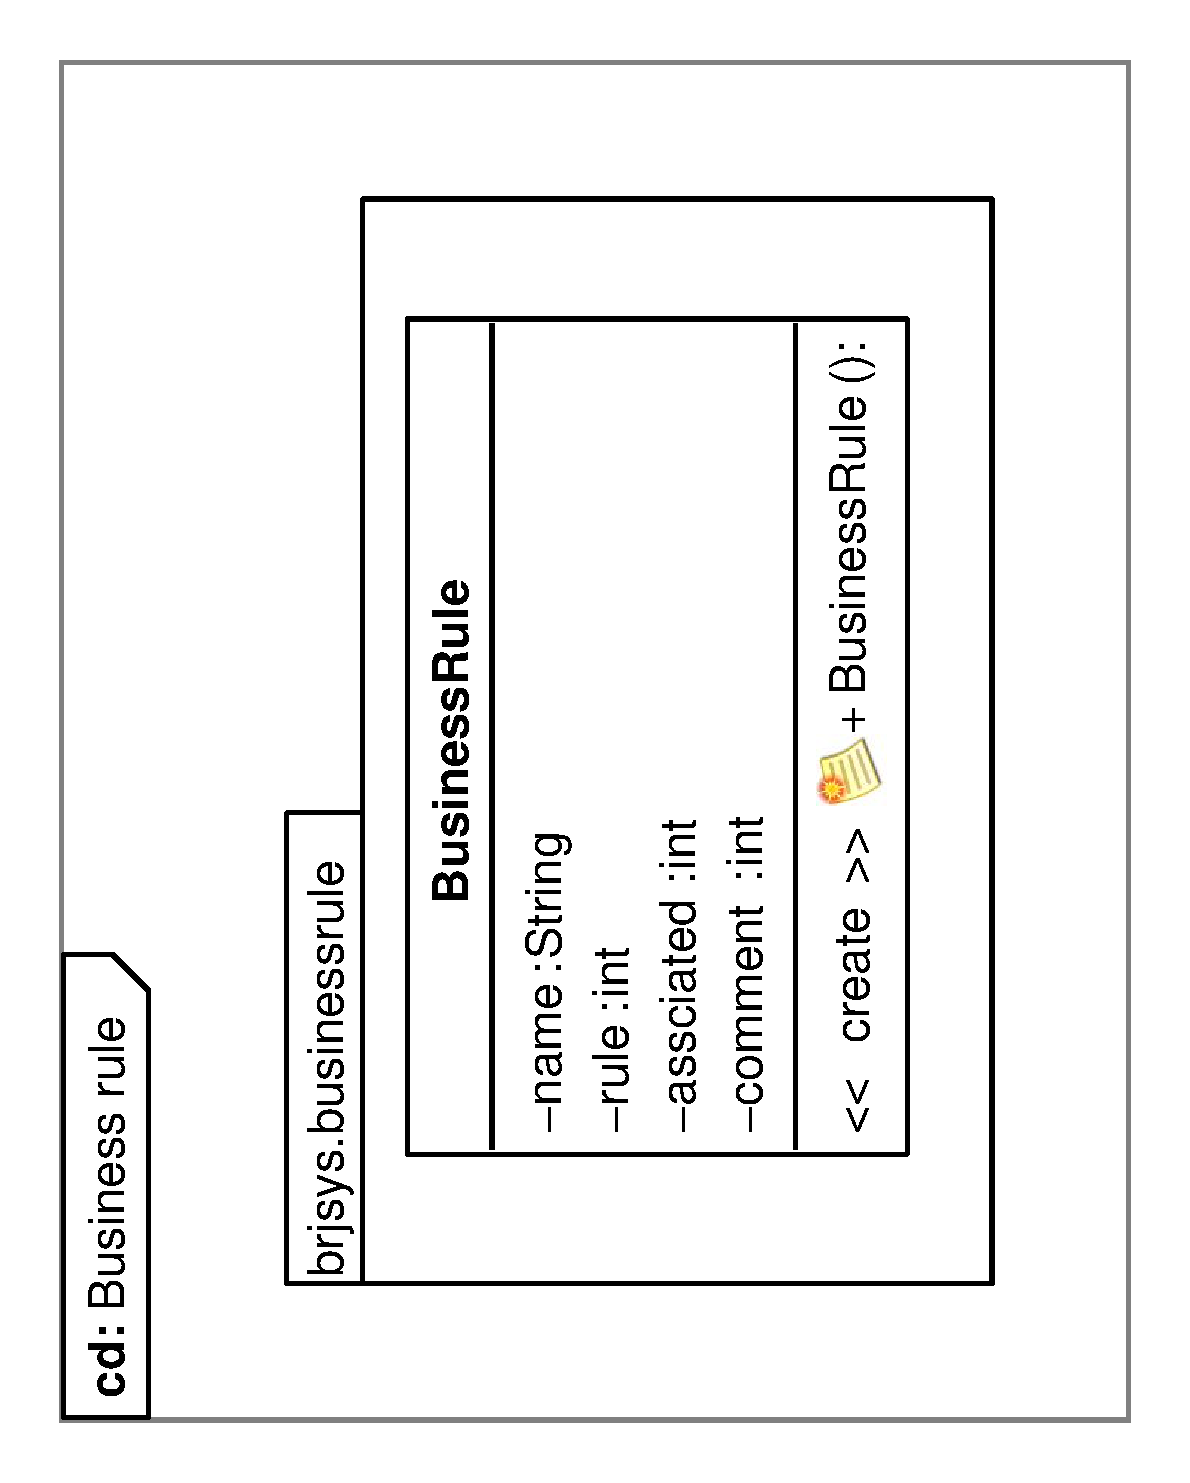
\includegraphics[width=0.5\textwidth, angle=-90]{DiagrammaClassi/Businessrule.eps}
\end{center}
\subsection{BusinessRule}
\subsubsection{Tipo, obiettivo e funzione del componente}
La componenete \BR rappresenta la \br che l'utente inserisce e vuole validare.
\subsubsection{Relazioni d'uso di altre componenti}
Nessuna.
\subsubsection{Interfacce con e relazioni di uso da altre componenti}
La componente GUI utilizza \BR nel caso in cui l'utente voglia inserire una nuova \br.
La componente Validator effettua la validazione di un istanza di \BR tramita la chamata del suo metodo validate().
\subsubsection{Attivit\`a svolte e dati trattati}
La componente contiene i campi dato Stringa per rappesentare una business rule ossia name, associatedObject, rule e comment, quest'ultima può non essere istanziata, vengono inoltre messi a disposizione il costruttore e il metodo ridefinito toString().
\begin{center}
\begin{tabular}{||p{6cm}||p{6cm}||} \hline
\hline
Attributo & Descrizione \\  \hline
+name:String &  Denota il nome della \br.\\ \hline
+associated:String & Denota il \bo assocato.\\ \hline
+rule:String &  Denota la \br scritta dall'utente e da validare.\\ \hline
+comment:String & Denota un commento opzionale che l'utente può associare a quella \br.\\ \hline
\end{tabular}
\end{center}
\begin{center}
\begin{tabular}{||p{6cm}||p{6cm}||} \hline
\hline
Metodo & Descrizione \\  \hline
BusinessRule(nameR: String , associatedR: String, ruleR: String, commentR: String) & Costruttore di BusinessRule.\\ \hline
\end{tabular}
\end{center}

\section{Comunicatore}
\subsection{Diagramma delle classi}
\begin{center}
%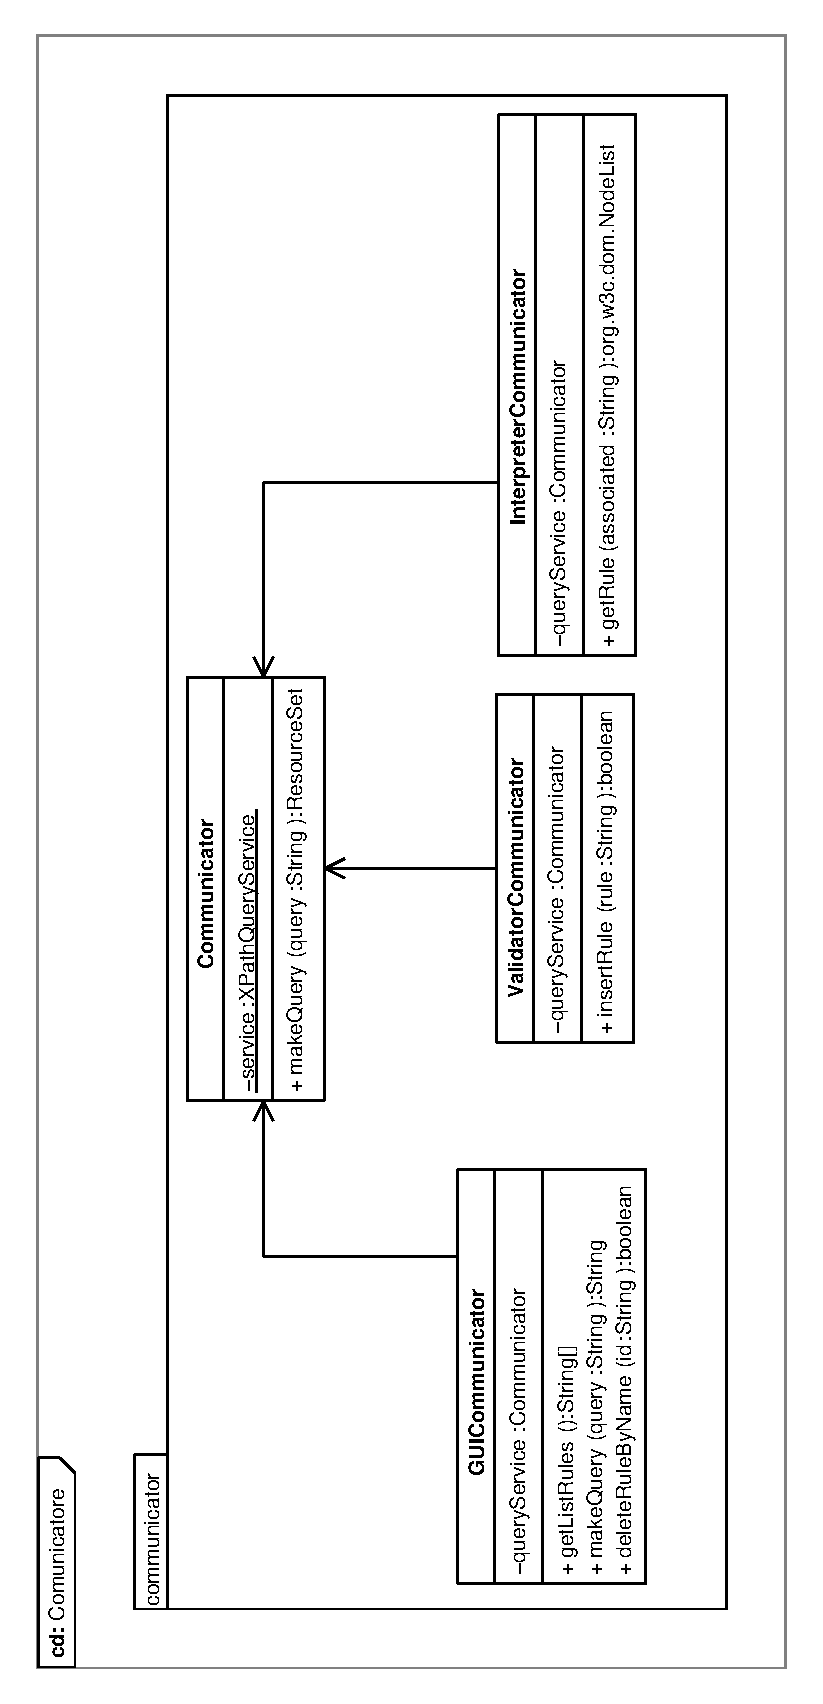
\includegraphics[width=0.5\textwidth, angle=-90]{DiagrammaClassi/Comunicatore.eps}
\end{center}
\subsection{Communicator}
\subsubsection{Tipo, obiettivo e funzione del componente}
Communicator fornisce alle componenti che la utilizzano la possibilit\`a di effettuare query di qualsiasi tipo al \re presente nel DBMS.
%Si comincia a parlare di eXist
Gli studi fatti su alcuni DBMS che manipolano dati XML hanno portato la HappyCode ad appoggiarsi su eXist, tramite le API messe a disposizione possiamo interagire con esso tramite costrutti java.
\subsubsection{Relazioni d'uso di altre componenti}
Communicator necessita di interagire con la componente esterna DBMS per interrogare il \re.
\subsubsection{Interfacce con e relazioni di uso da altre componenti}
Le componenti GUICommunicator, InterpreterCommunicator e ValidatorCommunicator necessitano di Communicator per potergli passare Query specifiche, le loro descrizioni sono trattate successivamente.
\subsubsection{Attivit\`a svolte e dati trattati}
Quando viene istanziata per la prima volta inizializza la connessione al DBMS tramite la definizione di una variabile statica che successivamente consente di interrogare il \re direttamente passandogli la stringa che rappresenta la query composta secondo le specifiche XQuery.
\begin{center}
\begin{tabular}{||p{6cm}||p{6cm}||} \hline
\hline
Attributo & Descrizione \\  \hline
\underline{-service:XPathQueryService} & Consente, se istanziato correttamente, di comunicare con risorse presenti su eXist, in particolare faremo in modo configurarlo in modo che faccia query solamente nel \re posizionato in una posizione specifica nel DBMS.\\ \hline
-correctUsername:String & Memorizza il corretto username utilizzato per l'accesso.\\ \hline
-correctPassword:String & memorizza la corretta password utilizzata per l'accesso.\\ \hline
\end{tabular}
\end{center}
\begin{center}
\begin{tabular}{||p{6cm}||p{6cm}||} \hline
\hline
Metodo & Descrizione \\  \hline
+Communicator(username: String, password: String) & Costruttore di Communicator. Nel caso si acceda alla classe per la prima volta durante l'esecuzione del programma si istanzierà l'attributo service, se la connessione \`e andata a buon fine gli attributi correctUsername e correctPassword verranno settati con i valori corrispondenti.Altrimeti se l'attributo service \`e gi\`a stato istanziato non si far\`a altro che assicurarsi che i parametri in ingresso al costruttore corrispondano a quelli presenti negli attributi.\\ \hline
+makeQuery(query:String) :ResourceSet & Metodo pubblico che ricevuto in ingresso una query scritta secondo le specifiche XQuery la esegue e ne restituisce il risultato.Si dovr\`a gestire il caso di query mal formata.
\end{tabular}
\end{center}

\subsection{GUICommunicator}
\subsubsection{Tipo, obiettivo e funzione del componente}
La componente contiene metodi necessari per modellare query di cancellazione(tramite operazioni XQuery Update) e di query di semplice interrogazione.
\subsubsection{Relazioni d'uso di altre componenti}
GUICommunicator utilizza la componente Communicator per accedere al \re ed interrogarlo.
\subsubsection{Interfacce con e relazioni di uso da altre componenti}
GUICommunicator viene messa in relazione con la componente GUI dalla quale riceve richieste di cancellazione e di querying.%si dice così no?
\subsubsection{Attivit\`a svolte e dati trattati}
GUICommunicator sar\`a strutturata nel seguente modo:
\begin{center}
\begin{tabular}{||p{6cm}||p{6cm}||} \hline
\hline
Attributo & Descrizione \\  \hline
-queryService:Communicator & Permette alla componente di colloquiare con eXist.\\ \hline
\end{tabular}
\end{center}
\begin{center}
\begin{tabular}{||p{6cm}||p{6cm}||} \hline
\hline
Metodo & Descrizione \\  \hline
+GUICommunicator(username: String, password: String) & Costruttore del componente, username e password saranno utilizzati per l'istanziazione di queryService. \\ \hline

+deleteRuleByName(id: String): boolean & Metodo per Cancellare un \br dato il suo identificativo, se la \br è stata trovata nel \re e dunque cancellata ritorner\`a \textit{true} altrimenti \textit{false}.\\ \hline

+makeQuery(query: String):String & Metodo per eseguire una query in XQuery, dovr\`o fare attenzione che la struttura della query non contenga istruzioni XQuery Update che permetterebbero all'utente di modificare a piacimento il \re rendendolo inconsistente.\\ \hline

+getListRules(): String[]& Metodo che ritorna informazioni riguardo le query scritte nel \re. in particolare l'array di ritorno avr\`a un elemento per \br nel \re ed ogni elemento conterr\`a il nome, la regola, il \bo associato e l'eventuale commento.\\ \hline
\end{tabular}
\end{center}

\subsection{InterpreterCommunicator}
\subsubsection{Tipo, obiettivo e funzione del componente}
InterpreterCommunicator contiene metodi necessari per rispondere a richieste di \br da parte di un interprete esterno.
\subsubsection{Relazioni d'uso di altre componenti}
InterpreterCommunicator utilizza la componente Communicator per accedere al \re ed interrogarlo.
\subsubsection{Interfacce con e relazioni di uso da altre componenti}
InterpreterCommunicator viene messa in relazione con l'interprete esterno dal quale riceve richieste di \brs associate ad un determinato \bo.
%Bisogna specificare le modalità di comunicazione
\subsubsection{Attivit\`a svolte e dati trattati}
InterpreterCommunicator offre il metodo getRule() per richiedere le \br associate al \bo.
\begin{center}
\begin{tabular}{||p{6cm}||p{6cm}||} \hline
\hline
Attributo & Descrizione \\  \hline
-queryService:Communicator & Permette alla componente di colloquiare con eXist.\\ \hline
\end{tabular}
\end{center}
\begin{center}
\begin{tabular}{||p{6cm}||p{6cm}||} \hline
\hline
Metodo & Descrizione \\  \hline
+InterpreterCommunicator( username: String, password: String) & Costuttore con funzionamento analogo a GUICommunicator.\\ \hline
+getRule(associated: String): NodeList & Dato in input un \bo ritorna tutte le \brs che sono associate ad esso, \\ \hline
\end{tabular}
\end{center}

\subsection{ValidatorCommunicator}
\subsubsection{Tipo, obiettivo e funzione del componente}
ValidatorCommunicator contiene metodi necessari per effettuare l'inserimento di una \br validata alla quale \`e stato effettuato il parsin in XML.
\subsubsection{Relazioni d'uso di altre componenti}
ValidatorCommunicator utilizza la componente Communicator per accedere al \re ed interrogarlo.
\subsubsection{Interfacce con e relazioni di uso da altre componenti}
ValidatorCommunicator viene messa in relazione con la componente Validator per effettuare l'inserimento.
\subsubsection{Attivit\`a svolte e dati trattati}
ValidatorCommunicator offre il metodi insertRule() per inserire la \br nel \re. L'inserimento avverr\`a soltanto se la \br ha un nome che non \`e ancora presente nel \re.
\begin{center}
\begin{tabular}{||p{6cm}||p{6cm}||} \hline
\hline
Attributo & Descrizione \\  \hline
-queryService:Communicator & Permette alla componente di colloquiare con eXist.\\ \hline
\end{tabular}
\end{center}
\begin{center}
\begin{tabular}{||p{6cm}||p{6cm}||} \hline
\hline
Metodo & Descrizione \\  \hline
ValidatorCommunicator(username: String, password: String) & Costruttore con comportamento analogo a GUICommunicator.\\ \hline
insertRule(rule: String, idRule: String): boolean & Inserisce la \br nel \re soltanto se il suo nome non \`e gi\`a presente. Se l'inserimento \`e andato a buon fine ritorner\`a \textit{true}.\\ \hline
\end{tabular}
\end{center}

\chapter{Appendice}
\section{Tracciamento della relazione componenti - requisiti}
\newpage

\tableofcontents
\end{document}
